\chapter{Appendix}
\label{cha:appendix}
\chaptermark{Appendix} 

\section{WASA2 Contributions}

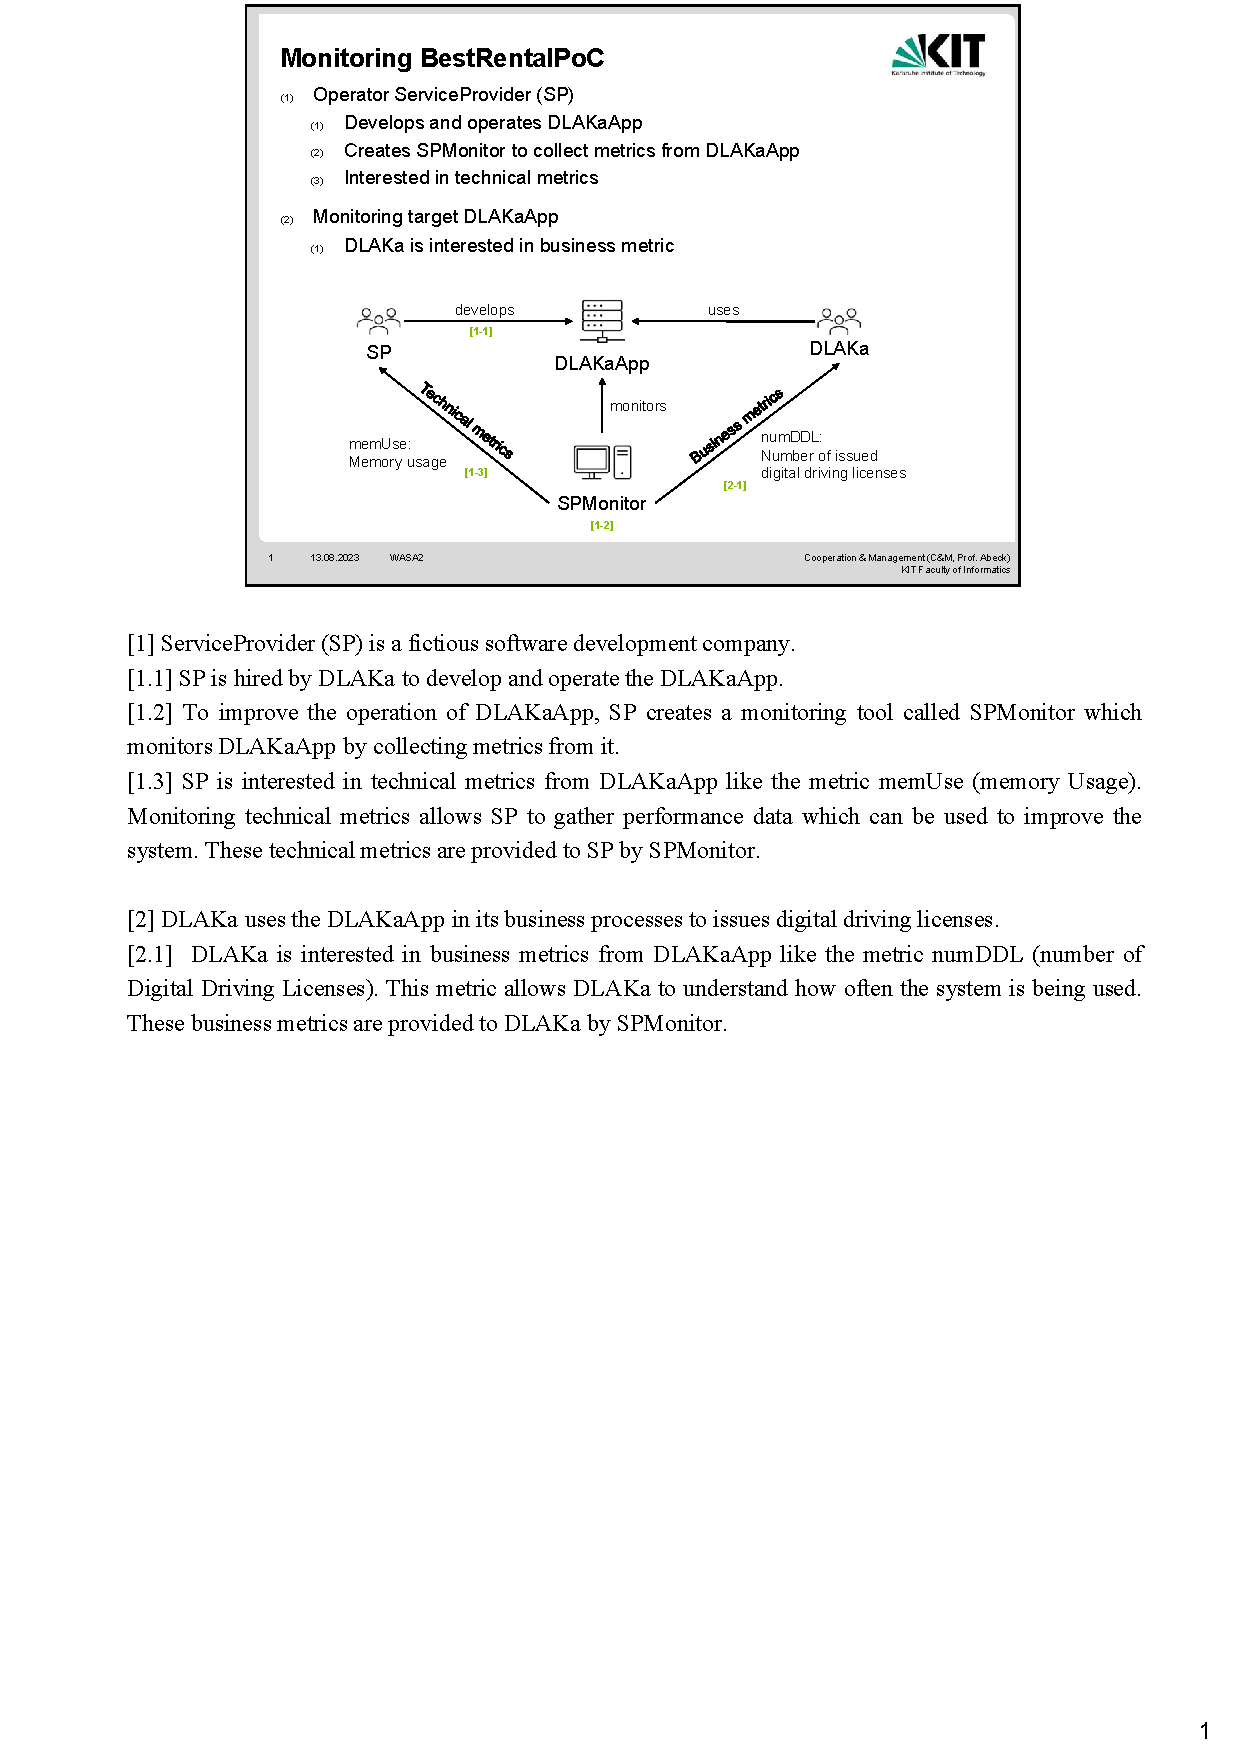
\includegraphics[height=\textheight]{pdfs/engbrocks_wasa2_monitoring.pdf}
\includepdf[pagecommand={\thispagestyle{plain}}, pages={2-last},height=\textheight]{pdfs/engbrocks_wasa2_monitoring.pdf}

\section{Snack and Learn}

The Snack and Learn talk by iCC (iC Consult) \cite{ICC-WEB} on the 29th of June 2023
titled Tools \& Templates - Unleashing the Power of Project Management Templates
discussed what project management templates are, their use cases, and their benefits.
The talk was held by Eric Bogard and Thomas Schuster.

The talk started with the introduction of the PM CoE (Project Management Center of Excellence)
which is a department at iCC that provides mentoring and support to project managers.
One of the ways the PM CoE supports project managers is by offering them a variety
of project management templates. Project management templates provide a standardized
basis for the processes and artifacts of project management. Examples include
templates for reports and planning. The templates offered by the PM CoE support
agile, waterfall, and hybrid processes and are available for all phases of
a project's lifecycle. All the templates offered by the PM CoE are related
to the tools with which they should be used. According to a statistic cited, only about 35\% of
projects are successful due to a variety of reasons. The goal of the project management
templates is the reduction of unknown risks by providing proven guidelines
for project management which leverage the combined company's expertise and experience.
This is shown in the nine reasons why, according to the PM CoE, project management templates
are important:
\begin{itemize}
      \item Effective use of project artifacts increases the probability of project success
      \item Reduces risk
      \item Starting point for new and/or less experienced PM's
      \item Consistency across the enterprise
      \item Save time - Why reinvent the wheel
      \item Reinforces best practices
      \item Empower you to do your job better
      \item Improves communication
      \item Tailorable to meet the needs of the project
\end{itemize}
The project management templates are based on successful projects and industry-based
practices. They are offered with iCC or customer branding and are available globally.
Because the PM CoE was only just created, a timeline was presented for when
the first templates would be published throughout the year, starting with the first
template in August and with the goal of publishing five templates by the end of the year.
PM CoE also announced a contest where participants could submit their proposals
for project management templates that will be considered in the future. The prizes
were not yet announced.
The talk ended by presenting the topic of the next Lunch and Learn: Project Health Monitor Tool
on the 28th of September 2023. Afterward, there was also a round of questions from audience members.

\section{Best Practice}

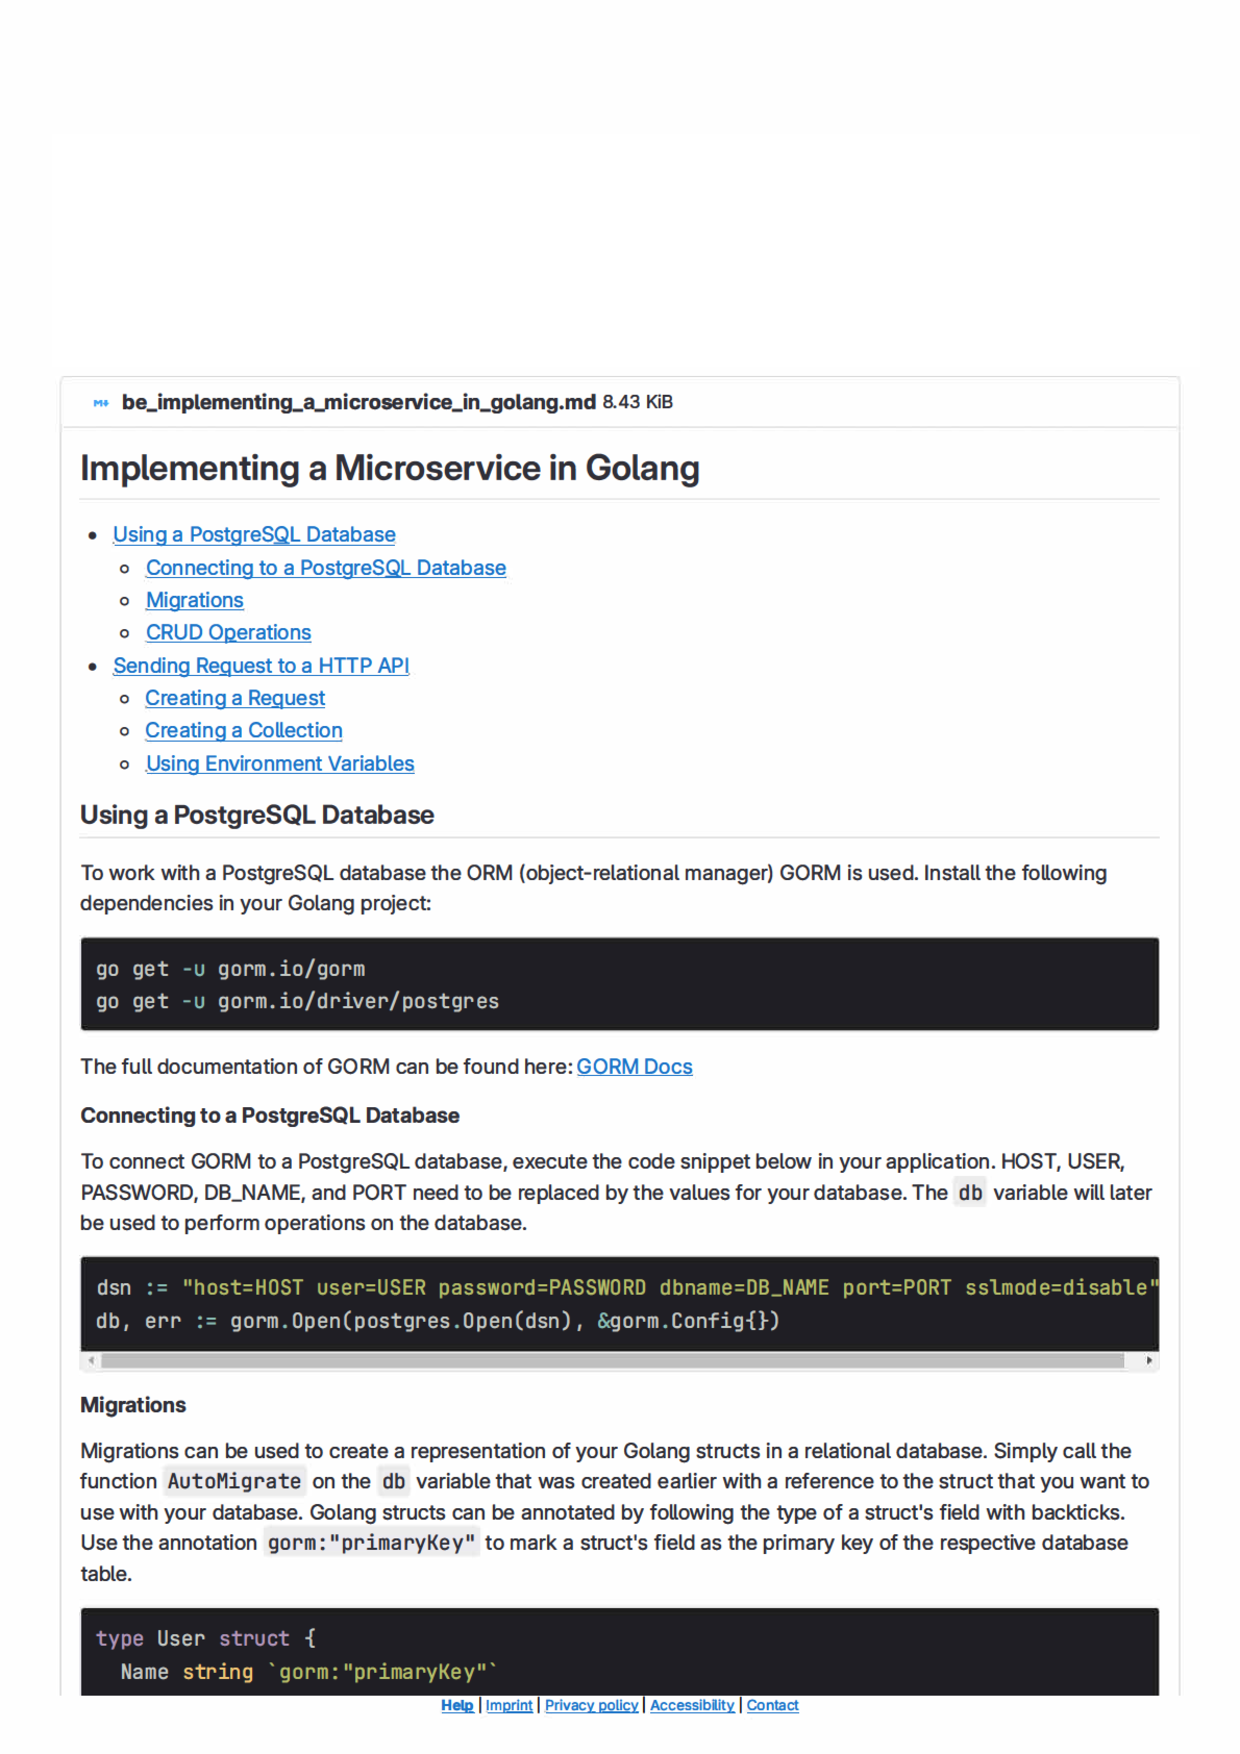
\includegraphics[height=\textheight]{pdfs/ume_be_implementing_a_microservice_in_golang.pdf}
\includepdf[pagecommand={\thispagestyle{plain}}, pages={2-last},height=\textheight]{pdfs/ume_be_implementing_a_microservice_in_golang.pdf}


%
% Bibliography
%
\makeatletter
\renewenvironment{thebibliography}[1]
     {\section{\bibname}
      \list{\@biblabel{\@arabic\c@enumiv}}
           {\settowidth\labelwidth{\@biblabel{#1}}
            \leftmargin\labelwidth
            \advance\leftmargin\labelsep
            \@openbib@code
            \usecounter{enumiv}%
            \let\p@enumiv\@empty
            \renewcommand\theenumiv{\@arabic\c@enumiv}}
      \sloppy
      \clubpenalty4000
      \@clubpenalty \clubpenalty
      \widowpenalty4000
      \sfcode`\.\@m}
     {\def\@noitemerr
       {\@latex@warning{Empty `thebibliography' environment}}%
      \endlist}
\makeatother

\bibliography{bt_engbrocks}

\bibliographystyle{cmnat}